%Author: Michael Bucher
\section{Host Client}

The host-client is a web-based application for event hosts to edit, track and create events. The application contains one component that is displayed and runs all the time. This component shows the active view and it contains a permanent navigation bar (Figure \ref{img:host-client-navbar}) that routes between the views of the application. The application is structured into five views. One of them, the event summary view, can be reached by clicking on an existing event card on the landing page and the other four can be reached through a sidebar. The navigation bar contains a button on the top left that toggles the sidebar (Figure \ref{img:host-client-sidebar}). It allows to route to the event list (landing page), a form to create a new event and as third option either a form to register as ID approver or, if already registered as ID approver, a form to approve an account manually.

\begin{figure}[H]
    \centering
    \fbox{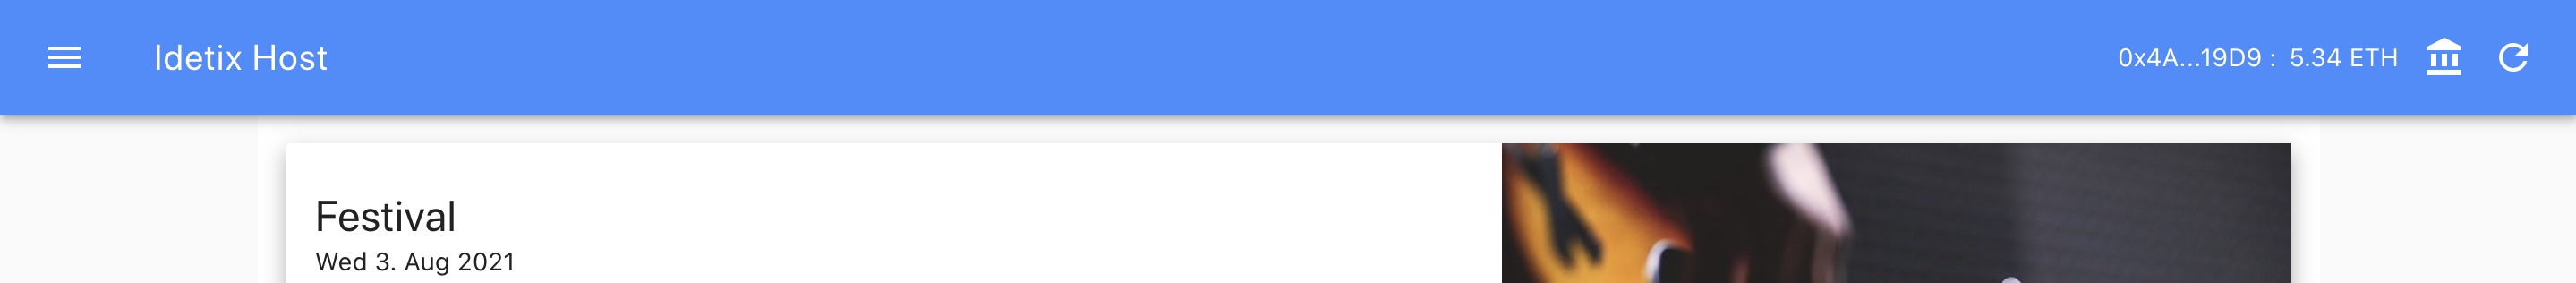
\includegraphics[width=15cm]{images/host-client-navbar-screenshot.png}}
    \caption{Host-client navigation bar \protect}
    \label{img:host-client-navbar}
\end{figure}

\begin{figure}[H]
    \centering
    \fbox{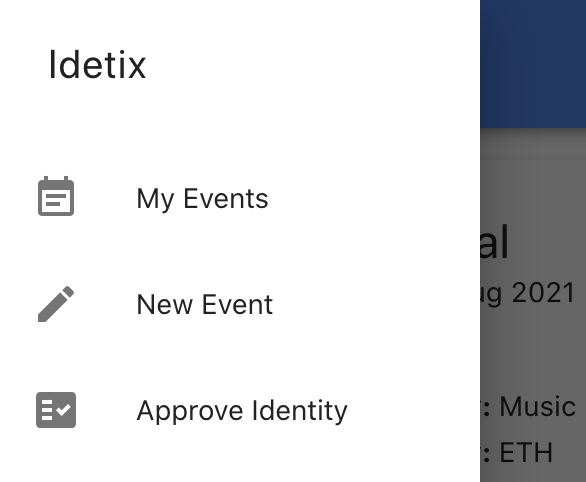
\includegraphics[width=5cm]{images/host-client-sidebar-screenshot.png}}
    \caption{Host-client sidebar \protect}
    \label{img:host-client-sidebar}
\end{figure}

When the application is started for the first time, the application needs to connect to a cryptocurrency wallet like Metamask\footnote{\href{https://metamask.io/}{https://metamask.io/}} to establish a connection to the Ethereum BC. The user is prompted to connect the wallet with their accounts to the website. As soon as the wallet is connected, the base component loads all registered ID approvers and all events that are owned by the active account in the wallet. Upon loading the main event data, the event list view is displayed, showing a list of the existing owned events. To create a new event, the event creation form is accessible through the navigation sidebar.

\subsection{Event Creation}\label{design:event-creation}
The event creation form component contains various input fields to set up a new event. There are parts that are required, like the title, location, date, description and the aftermarket granularity. Only when those required parts are filled, a button is shown at the bottom to create the event. An ID approver is not required based on the design of the event factory contract. Further, an image, a website or twitter account are also optional.

When selecting an ID approver, their selector is automatically filled with the existing ID approvers that are registered on the identity SC. When an ID approver is selected, the level selector on its right is updated with the according methods. Further, to get more information for the selected ID approver, the question mark icon on the right opens a dialog window that explains the involvement of an ID approver to this event and also leads to a dialog that provides an overview of the ID approver, like its website, twitter and what identity verification methods are supported.

Further, the website and twitter input fields show the status of the trust certificate (see Section \ref{section:social-trust-certificates}) check for the given input and the active account. This way, a correct integration of a host's certificates can be checked. Finally, upon creating an event, the user is routed back to the event list.

\begin{figure}[H]
    \centering
    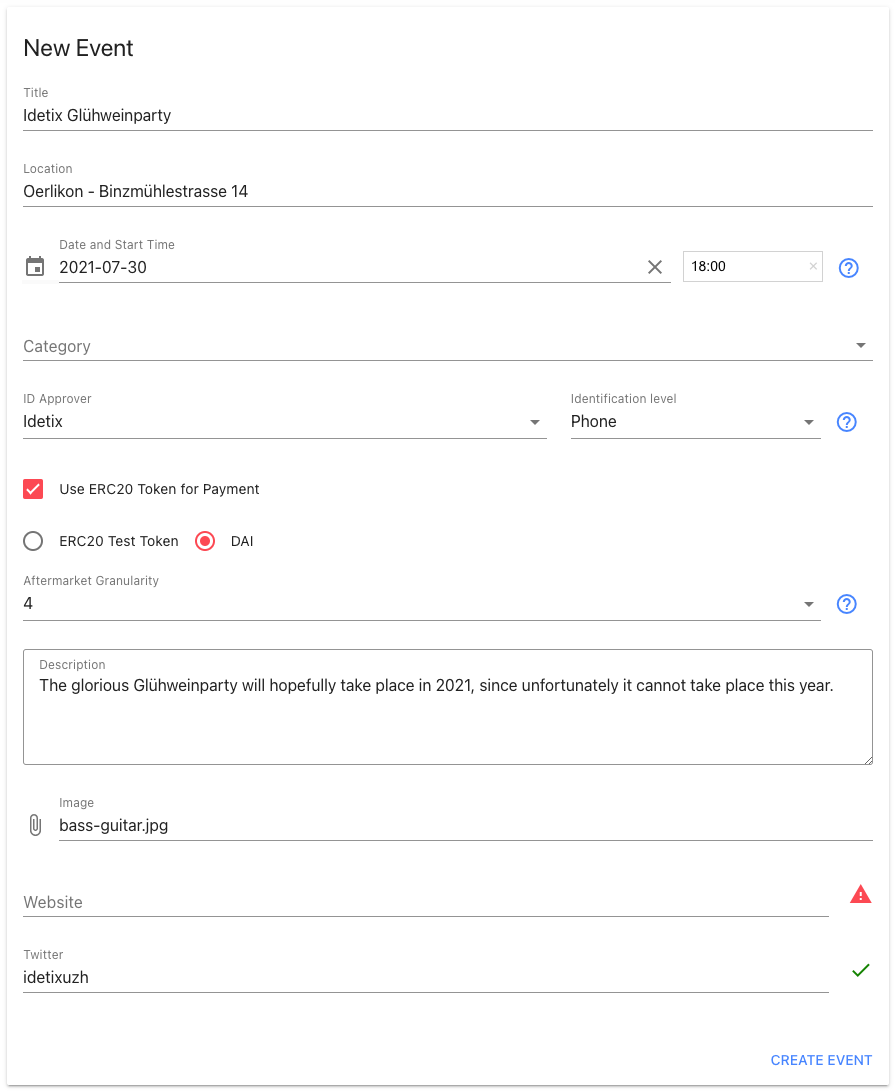
\includegraphics[width=15cm]{images/host-event-form.png}
    \caption{Event creation form \protect}
    \label{img:host-event-form}
\end{figure}

\subsection{Event List}
The event list is a simple view that contains a list of event cards. These event cards contain the metadata for the according event and some information directly fetched from the BC, i.e. the maximal number of tickets per person, the currency, or the ID approver that is required to buy a ticket. For more information about an event, a click on the card routes to the event summary view.

\subsection{Event Summary}
The event summary view (Figure \ref{img:host-event-summary}) contains multiple components that offer an overview of the event, its tickets, and their states. A slightly reconfigured event card to the card in the event list is shown on top. Here it also shows the event contract address and an edit button. Either the metadata or the maximal number of tickets per person can be changed. Upon clicking the edit button, the host is prompted what to change and the according component is shown to make such a change.
When editing the metadata, an event creation form is displayed that is filled with the current metadata. This form can be edited and then submitted. In the form, only the image input is not filled out with the current data, since it is stored in a Base64 representation. If no new image is uploaded in this input field, the current image is just used again. After a change to the event, the event summary is shown again with the updated data.

\begin{figure}[H]
    \centering
    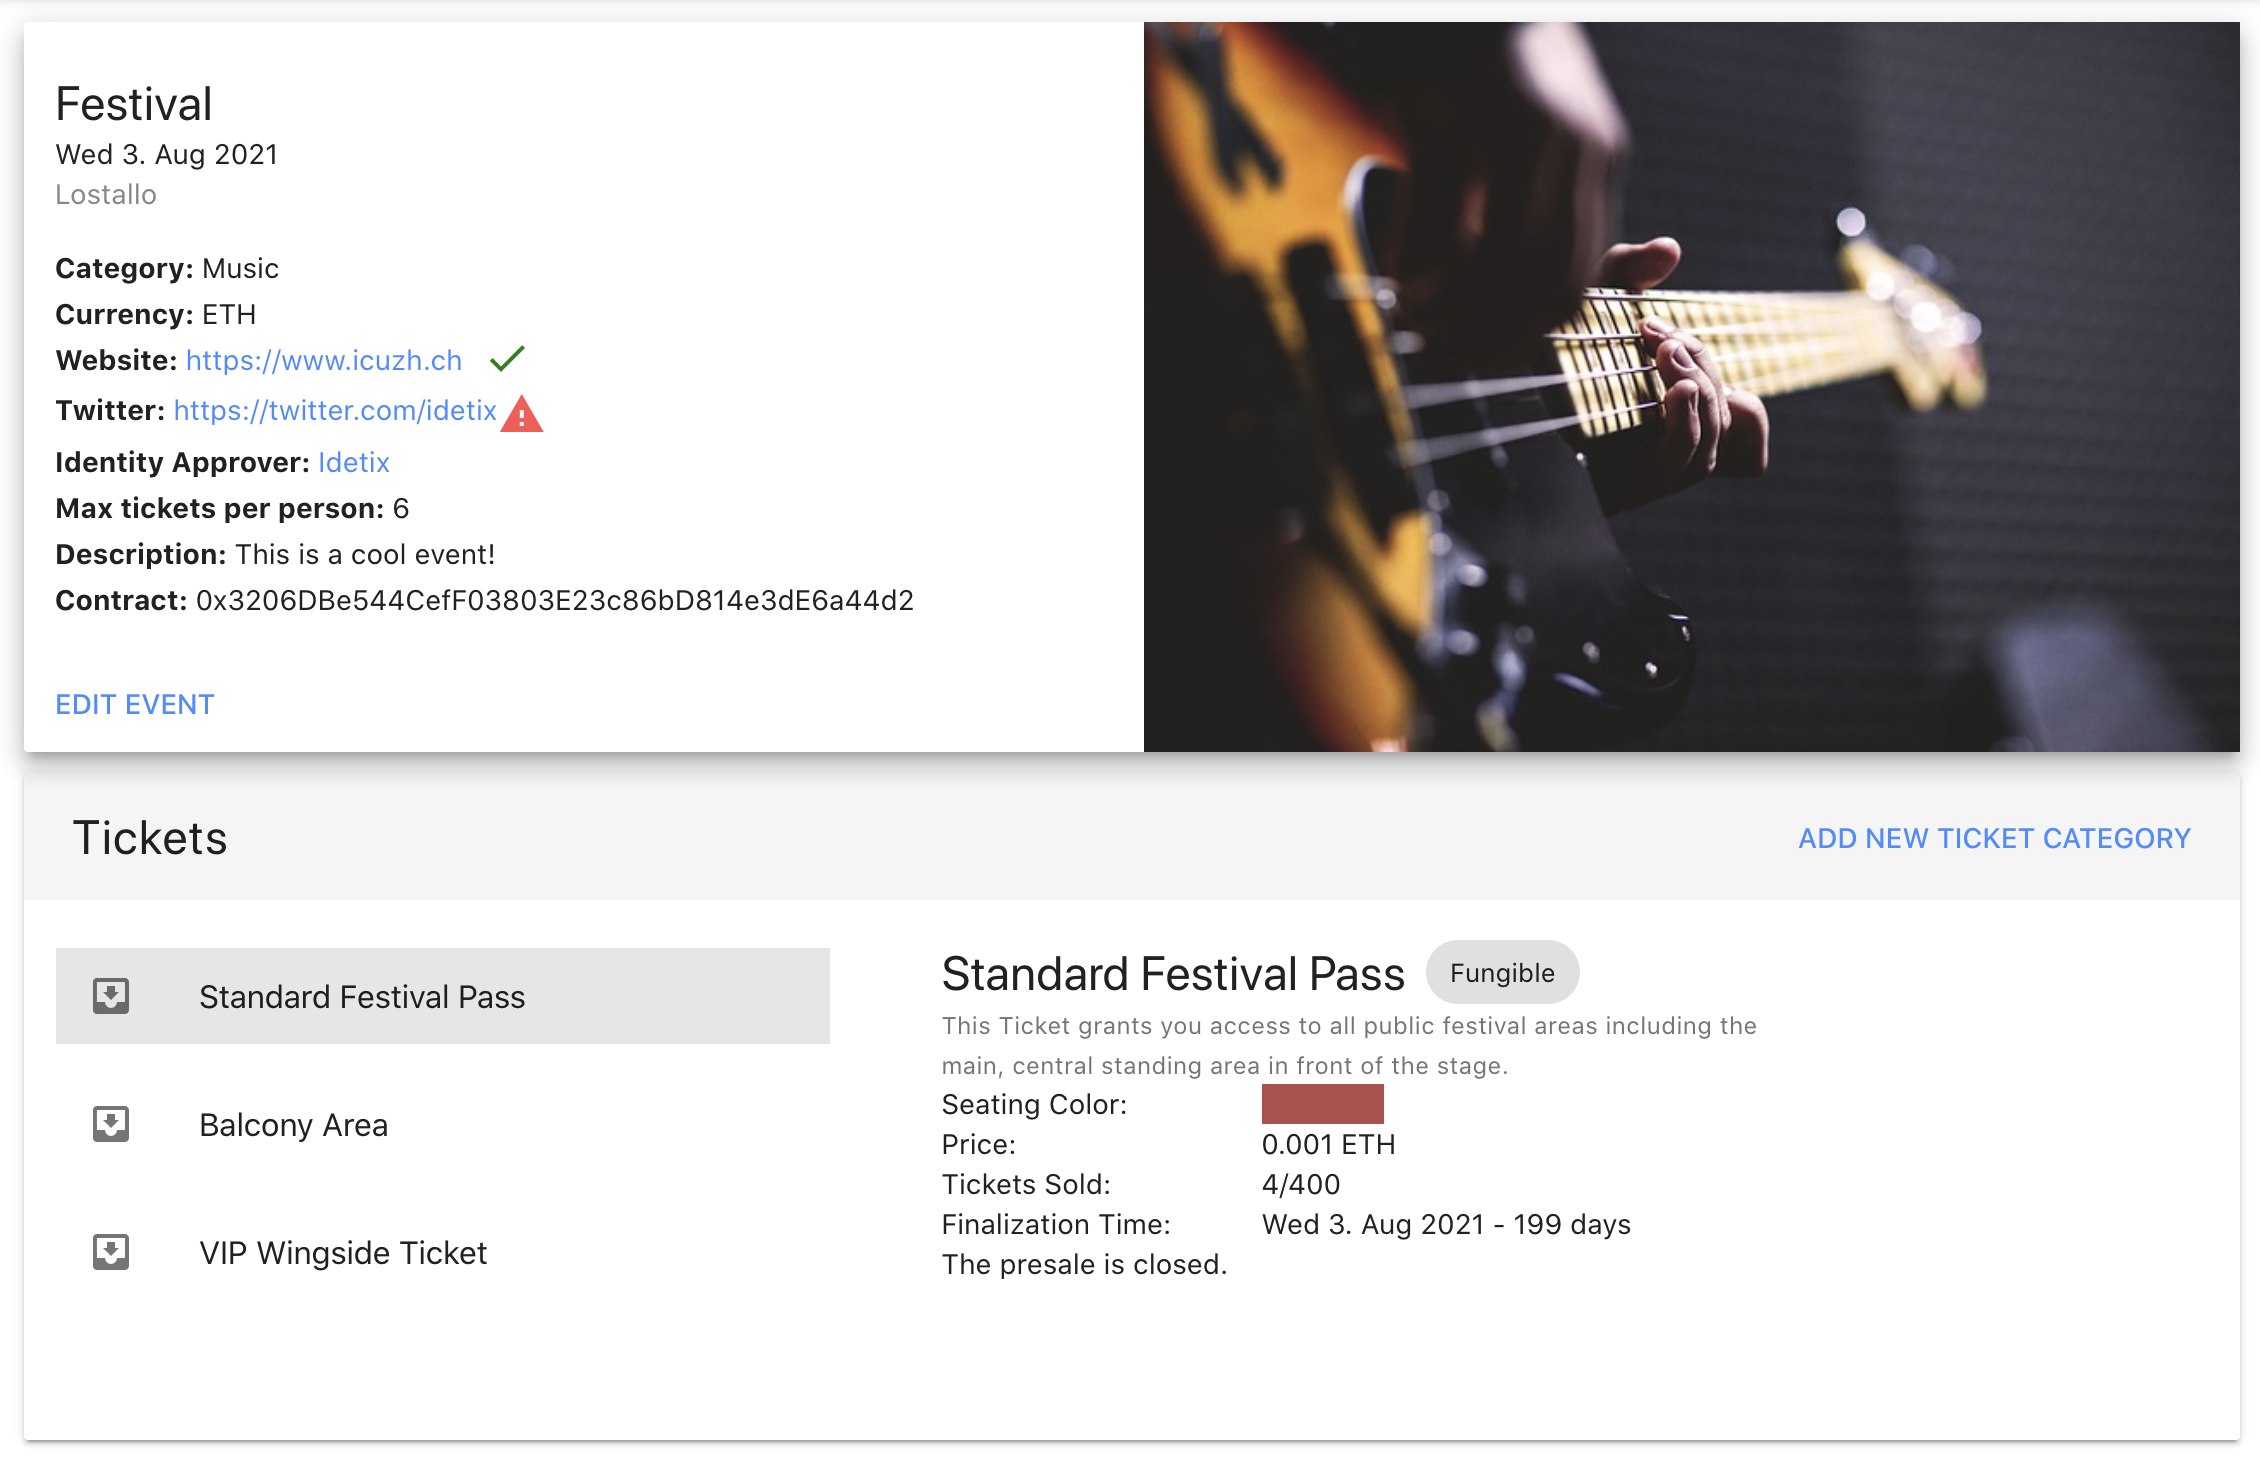
\includegraphics[width=14cm]{images/host-event-summary.png}
    \caption{Event summary view \protect}
    \label{img:host-event-summary}
\end{figure}

Below the event card, the tickets of the event are summarized. On the left is a list of ticket types that exist for that event and when selecting a ticket, the information about this ticket is shown on the right. This information contains data from the BC and the metadata that is fetched from IPFS. It shows details such as whether the ticket is fungible or non-fungible, the price, the amount of tickets that have already been sold and the finalization time. This finalization time specifies the time, when tickets can no longer be bought or sold.
Tickets with a presale further show the status of this presale. Either, the presale has already passed, or otherwise, an estimated time is shown, when the presale presumably will end.

Additional to that, the BC information of a ticket and the ticket's metadata which is stored on IPFS is shown, i.e. title, description and the seating color. The latter may then directly be used to visualise what seats this type contains on the seating plan that is shown directly below.

To add a new ticket type to the event, this ticket summary component holds a button on the top right, which opens a ticket form. In this form, the host can set the metadata for a new ticket type as desired. There are just a few restrictions that arise from properties of the event or already existing ticket types, such as already used seats in the seating plan component, that may not be used for another ticket type. When saving a category, the selected seats of the seating plan component together with the filled out information in the ticket form are pre-saved and added to a list below as in Figure \ref{img:host-seating-plan}. A new submit button is now shown. With this button, the ticket types are created in one invocation on the event contract. Given the design choice in the SCs, ticket types with a presale require a separate invocation. This means, that if the pre-saved tickets contain both tickets with a presale and tickets without a presale, two invocations are required.

\begin{figure}[H]
    \centering
    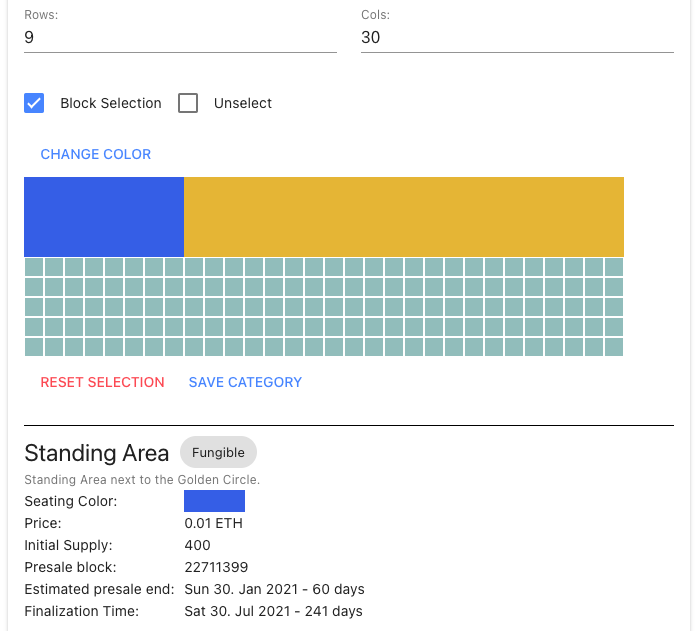
\includegraphics[width=14cm]{images/host-seating-plan.png}
    \caption{Seating plan \protect}
    \label{img:host-seating-plan}
\end{figure}

Currently, changes to the ticket metadata are allowed in our SCs. However, since in our design the seat mapping of a ticket type is also stored in the metadata, we do not provide such functionality in the host-client to prevent duplicated seats in the seating plan. This is addressed further as a potential future work task (see Section \ref{future-work-ticket-metadata-change}).

\subsection{ID Approver Registration and Identity Approval}
As extension to the host-client application, two views are included that support a basic interaction with the identity SC. The ID approver registration view contains a form to easily register as an ID approver with their supported methods, website and twitter. The website and twitter input fields also trigger a check for the trust certificates as in the event creation form. Once an ID approver is registered, the identity approval form allows to easily store the verification level of an account on the identity SC.
